
%% bare_conf.tex
%% V1.3
%% 2007/01/11
%% by Michael Shell
%% See:
%% http://www.michaelshell.org/
%% for current contact information.
%%
%% This is a skeleton file demonstrating the use of IEEEtran.cls
%% (requires IEEEtran.cls version 1.7 or later) with an IEEE conference paper.
%%
%% Support sites:
%% http://www.michaelshell.org/tex/ieeetran/
%% http://www.ctan.org/tex-archive/macros/latex/contrib/IEEEtran/
%% and
%% http://www.ieee.org/

%%*************************************************************************
%% Legal Notice:
%% This code is offered as-is without any warranty either expressed or
%% implied; without even the implied warranty of MERCHANTABILITY or
%% FITNESS FOR A PARTICULAR PURPOSE! 
%% User assumes all risk.
%% In no event shall IEEE or any contributor to this code be liable for
%% any damages or losses, including, but not limited to, incidental,
%% consequential, or any other damages, resulting from the use or misuse
%% of any information contained here.
%%
%% All comments are the opinions of their respective authors and are not
%% necessarily endorsed by the IEEE.
%%
%% This work is distributed under the LaTeX Project Public License (LPPL)
%% ( http://www.latex-project.org/ ) version 1.3, and may be freely used,
%% distributed and modified. A copy of the LPPL, version 1.3, is included
%% in the base LaTeX documentation of all distributions of LaTeX released
%% 2003/12/01 or later.
%% Retain all contribution notices and credits.
%% ** Modified files should be clearly indicated as such, including  **
%% ** renaming them and changing author support contact information. **
%%
%% File list of work: IEEEtran.cls, IEEEtran_HOWTO.pdf, bare_adv.tex,
%%                    bare_conf.tex, bare_jrnl.tex, bare_jrnl_compsoc.tex
%%*************************************************************************

% *** Authors should verify (and, if needed, correct) their LaTeX system  ***
% *** with the testflow diagnostic prior to trusting their LaTeX platform ***
% *** with production work. IEEE's font choices can trigger bugs that do  ***
% *** not appear when using other class files.                            ***
% The testflow support page is at:
% http://www.michaelshell.org/tex/testflow/



% Note that the a4paper option is mainly intended so that authors in
% countries using A4 can easily print to A4 and see how their papers will
% look in print - the typesetting of the document will not typically be
% affected with changes in paper size (but the bottom and side margins will).
% Use the testflow package mentioned above to verify correct handling of
% both paper sizes by the user's LaTeX system.
%
% Also note that the "draftcls" or "draftclsnofoot", not "draft", option
% should be used if it is desired that the figures are to be displayed in
% draft mode.
%
\documentclass[conference]{IEEEtran}
% Add the compsoc option for Computer Society conferences.
%
% If IEEEtran.cls has not been installed into the LaTeX system files,
% manually specify the path to it like:
% \documentclass[conference]{../sty/IEEEtran}





% Some very useful LaTeX packages include:
% (uncomment the ones you want to load)


% *** MISC UTILITY PACKAGES ***
%
%\usepackage{ifpdf}
% Heiko Oberdiek's ifpdf.sty is very useful if you need conditional
% compilation based on whether the output is pdf or dvi.
% usage:
% \ifpdf
%   % pdf code
% \else
%   % dvi code
% \fi
% The latest version of ifpdf.sty can be obtained from:
% http://www.ctan.org/tex-archive/macros/latex/contrib/oberdiek/
% Also, note that IEEEtran.cls V1.7 and later provides a builtin
% \ifCLASSINFOpdf conditional that works the same way.
% When switching from latex to pdflatex and vice-versa, the compiler may
% have to be run twice to clear warning/error messages.






% *** CITATION PACKAGES ***
%
%\usepackage{cite}
% cite.sty was written by Donald Arseneau
% V1.6 and later of IEEEtran pre-defines the format of the cite.sty package
% \cite{} output to follow that of IEEE. Loading the cite package will
% result in citation numbers being automatically sorted and properly
% "compressed/ranged". e.g., [1], [9], [2], [7], [5], [6] without using
% cite.sty will become [1], [2], [5]--[7], [9] using cite.sty. cite.sty's
% \cite will automatically add leading space, if needed. Use cite.sty's
% noadjust option (cite.sty V3.8 and later) if you want to turn this off.
% cite.sty is already installed on most LaTeX systems. Be sure and use
% version 4.0 (2003-05-27) and later if using hyperref.sty. cite.sty does
% not currently provide for hyperlinked citations.
% The latest version can be obtained at:
% http://www.ctan.org/tex-archive/macros/latex/contrib/cite/
% The documentation is contained in the cite.sty file itself.






% *** GRAPHICS RELATED PACKAGES ***
%
\ifCLASSINFOpdf
   \usepackage[pdftex]{graphicx}
  % declare the path(s) where your graphic files are
   \graphicspath{{images/}}
  % and their extensions so you won't have to specify these with
  % every instance of \includegraphics
   \DeclareGraphicsExtensions{.pdf,.jpeg,.png}
\else
  % or other class option (dvipsone, dvipdf, if not using dvips). graphicx
  % will default to the driver specified in the system graphics.cfg if no
  % driver is specified.
  % \usepackage[dvips]{graphicx}
  % declare the path(s) where your graphic files are
  % \graphicspath{{../eps/}}
  % and their extensions so you won't have to specify these with
  % every instance of \includegraphics
  % \DeclareGraphicsExtensions{.eps}
\fi
% graphicx was written by David Carlisle and Sebastian Rahtz. It is
% required if you want graphics, photos, etc. graphicx.sty is already
% installed on most LaTeX systems. The latest version and documentation can
% be obtained at: 
% http://www.ctan.org/tex-archive/macros/latex/required/graphics/
% Another good source of documentation is "Using Imported Graphics in
% LaTeX2e" by Keith Reckdahl which can be found as epslatex.ps or
% epslatex.pdf at: http://www.ctan.org/tex-archive/info/
%
% latex, and pdflatex in dvi mode, support graphics in encapsulated
% postscript (.eps) format. pdflatex in pdf mode supports graphics
% in .pdf, .jpeg, .png and .mps (metapost) formats. Users should ensure
% that all non-photo figures use a vector format (.eps, .pdf, .mps) and
% not a bitmapped formats (.jpeg, .png). IEEE frowns on bitmapped formats
% which can result in "jaggedy"/blurry rendering of lines and letters as
% well as large increases in file sizes.
%
% You can find documentation about the pdfTeX application at:
% http://www.tug.org/applications/pdftex





% *** MATH PACKAGES ***
%
%\usepackage[cmex10]{amsmath}
% A popular package from the American Mathematical Society that provides
% many useful and powerful commands for dealing with mathematics. If using
% it, be sure to load this package with the cmex10 option to ensure that
% only type 1 fonts will utilized at all point sizes. Without this option,
% it is possible that some math symbols, particularly those within
% footnotes, will be rendered in bitmap form which will result in a
% document that can not be IEEE Xplore compliant!
%
% Also, note that the amsmath package sets \interdisplaylinepenalty to 10000
% thus preventing page breaks from occurring within multiline equations. Use:
%\interdisplaylinepenalty=2500
% after loading amsmath to restore such page breaks as IEEEtran.cls normally
% does. amsmath.sty is already installed on most LaTeX systems. The latest
% version and documentation can be obtained at:
% http://www.ctan.org/tex-archive/macros/latex/required/amslatex/math/





% *** SPECIALIZED LIST PACKAGES ***
%
%\usepackage{algorithmic}
% algorithmic.sty was written by Peter Williams and Rogerio Brito.
% This package provides an algorithmic environment fo describing algorithms.
% You can use the algorithmic environment in-text or within a figure
% environment to provide for a floating algorithm. Do NOT use the algorithm
% floating environment provided by algorithm.sty (by the same authors) or
% algorithm2e.sty (by Christophe Fiorio) as IEEE does not use dedicated
% algorithm float types and packages that provide these will not provide
% correct IEEE style captions. The latest version and documentation of
% algorithmic.sty can be obtained at:
% http://www.ctan.org/tex-archive/macros/latex/contrib/algorithms/
% There is also a support site at:
% http://algorithms.berlios.de/index.html
% Also of interest may be the (relatively newer and more customizable)
% algorithmicx.sty package by Szasz Janos:
% http://www.ctan.org/tex-archive/macros/latex/contrib/algorithmicx/




% *** ALIGNMENT PACKAGES ***
%
%\usepackage{array}
% Frank Mittelbach's and David Carlisle's array.sty patches and improves
% the standard LaTeX2e array and tabular environments to provide better
% appearance and additional user controls. As the default LaTeX2e table
% generation code is lacking to the point of almost being broken with
% respect to the quality of the end results, all users are strongly
% advised to use an enhanced (at the very least that provided by array.sty)
% set of table tools. array.sty is already installed on most systems. The
% latest version and documentation can be obtained at:
% http://www.ctan.org/tex-archive/macros/latex/required/tools/


%\usepackage{mdwmath}
%\usepackage{mdwtab}
% Also highly recommended is Mark Wooding's extremely powerful MDW tools,
% especially mdwmath.sty and mdwtab.sty which are used to format equations
% and tables, respectively. The MDWtools set is already installed on most
% LaTeX systems. The lastest version and documentation is available at:
% http://www.ctan.org/tex-archive/macros/latex/contrib/mdwtools/


% IEEEtran contains the IEEEeqnarray family of commands that can be used to
% generate multiline equations as well as matrices, tables, etc., of high
% quality.


%\usepackage{eqparbox}
% Also of notable interest is Scott Pakin's eqparbox package for creating
% (automatically sized) equal width boxes - aka "natural width parboxes".
% Available at:
% http://www.ctan.org/tex-archive/macros/latex/contrib/eqparbox/





% *** SUBFIGURE PACKAGES ***
%\usepackage[tight,footnotesize]{subfigure}
% subfigure.sty was written by Steven Douglas Cochran. This package makes it
% easy to put subfigures in your figures. e.g., "Figure 1a and 1b". For IEEE
% work, it is a good idea to load it with the tight package option to reduce
% the amount of white space around the subfigures. subfigure.sty is already
% installed on most LaTeX systems. The latest version and documentation can
% be obtained at:
% http://www.ctan.org/tex-archive/obsolete/macros/latex/contrib/subfigure/
% subfigure.sty has been superceeded by subfig.sty.



%\usepackage[caption=false]{caption}
%\usepackage[font=footnotesize]{subfig}
% subfig.sty, also written by Steven Douglas Cochran, is the modern
% replacement for subfigure.sty. However, subfig.sty requires and
% automatically loads Axel Sommerfeldt's caption.sty which will override
% IEEEtran.cls handling of captions and this will result in nonIEEE style
% figure/table captions. To prevent this problem, be sure and preload
% caption.sty with its "caption=false" package option. This is will preserve
% IEEEtran.cls handing of captions. Version 1.3 (2005/06/28) and later 
% (recommended due to many improvements over 1.2) of subfig.sty supports
% the caption=false option directly:
%\usepackage[caption=false,font=footnotesize]{subfig}
%
% The latest version and documentation can be obtained at:
% http://www.ctan.org/tex-archive/macros/latex/contrib/subfig/
% The latest version and documentation of caption.sty can be obtained at:
% http://www.ctan.org/tex-archive/macros/latex/contrib/caption/




% *** FLOAT PACKAGES ***
%
%\usepackage{fixltx2e}
% fixltx2e, the successor to the earlier fix2col.sty, was written by
% Frank Mittelbach and David Carlisle. This package corrects a few problems
% in the LaTeX2e kernel, the most notable of which is that in current
% LaTeX2e releases, the ordering of single and double column floats is not
% guaranteed to be preserved. Thus, an unpatched LaTeX2e can allow a
% single column figure to be placed prior to an earlier double column
% figure. The latest version and documentation can be found at:
% http://www.ctan.org/tex-archive/macros/latex/base/



%\usepackage{stfloats}
% stfloats.sty was written by Sigitas Tolusis. This package gives LaTeX2e
% the ability to do double column floats at the bottom of the page as well
% as the top. (e.g., "\begin{figure*}[!b]" is not normally possible in
% LaTeX2e). It also provides a command:
%\fnbelowfloat
% to enable the placement of footnotes below bottom floats (the standard
% LaTeX2e kernel puts them above bottom floats). This is an invasive package
% which rewrites many portions of the LaTeX2e float routines. It may not work
% with other packages that modify the LaTeX2e float routines. The latest
% version and documentation can be obtained at:
% http://www.ctan.org/tex-archive/macros/latex/contrib/sttools/
% Documentation is contained in the stfloats.sty comments as well as in the
% presfull.pdf file. Do not use the stfloats baselinefloat ability as IEEE
% does not allow \baselineskip to stretch. Authors submitting work to the
% IEEE should note that IEEE rarely uses double column equations and
% that authors should try to avoid such use. Do not be tempted to use the
% cuted.sty or midfloat.sty packages (also by Sigitas Tolusis) as IEEE does
% not format its papers in such ways.





% *** PDF, URL AND HYPERLINK PACKAGES ***
%
%\usepackage{url}
% url.sty was written by Donald Arseneau. It provides better support for
% handling and breaking URLs. url.sty is already installed on most LaTeX
% systems. The latest version can be obtained at:
% http://www.ctan.org/tex-archive/macros/latex/contrib/misc/
% Read the url.sty source comments for usage information. Basically,
% \url{my_url_here}.





% *** Do not adjust lengths that control margins, column widths, etc. ***
% *** Do not use packages that alter fonts (such as pslatex).         ***
% There should be no need to do such things with IEEEtran.cls V1.6 and later.
% (Unless specifically asked to do so by the journal or conference you plan
% to submit to, of course. )


% correct bad hyphenation here
\hyphenation{op-tical net-works semi-conduc-tor}


\begin{document}
%
% paper title
% can use linebreaks \\ within to get better formatting as desired
\title{Decentralized Collision Avoidance Framework for Unmanned Aerial Vehicles}


% author names and affiliations
% use a multiple column layout for up to three different
% affiliations
\author{\IEEEauthorblockN{Andrew Cunningham}
\IEEEauthorblockA{
Rensselaer Polytechnic Institute\\
Troy, New York\\
cunnia3@rpi.edu}
\and
\IEEEauthorblockN{Victoria Wu}
\IEEEauthorblockA{
University of Missouri - Kansas City\\
Kansas City, Missouri\\
vcw7c5@mail.umkc.edu}
\and
\IEEEauthorblockN{Saad Biaz}
\IEEEauthorblockA{
Auburn University\\
Auburn, Alabama\\
biazsaa@auburn.edu}
\and
\IEEEauthorblockN{David Jones}
\IEEEauthorblockA{
Auburn University\\
Auburn, Alabama\\
dhj0001@auburn.edu
}

}

% conference papers do not typically use \thanks and this command
% is locked out in conference mode. If really needed, such as for
% the acknowledgment of grants, issue a \IEEEoverridecommandlockouts
% after \documentclass

% for over three affiliations, or if they all won't fit within the width
% of the page, use this alternative format:
% 
%\author{\IEEEauthorblockN{Michael Shell\IEEEauthorrefmark{1},
%Homer Simpson\IEEEauthorrefmark{2},
%James Kirk\IEEEauthorrefmark{3}, 
%Montgomery Scott\IEEEauthorrefmark{3} and
%Eldon Tyrell\IEEEauthorrefmark{4}}
%\IEEEauthorblockA{\IEEEauthorrefmark{1}School of Electrical and Computer Engineering\\
%Georgia Institute of Technology,
%Atlanta, Georgia 30332--0250\\ Email: see http://www.michaelshell.org/contact.html}
%\IEEEauthorblockA{\IEEEauthorrefmark{2}Twentieth Century Fox, Springfield, USA\\
%Email: homer@thesimpsons.com}
%\IEEEauthorblockA{\IEEEauthorrefmark{3}Starfleet Academy, San Francisco, California 96678-2391\\
%Telephone: (800) 555--1212, Fax: (888) 555--1212}
%\IEEEauthorblockA{\IEEEauthorrefmark{4}Tyrell Inc., 123 Replicant Street, Los Angeles, California 90210--4321}}




% use for special paper notices
%\IEEEspecialpapernotice{(Invited Paper)}




% make the title area
\maketitle


\begin{abstract}
%\boldmath
Collision avoidance for unmanned aerial vehicles (UAVs) is a vital issue when using multiple drones. Decentralized collision avoidance algorithms allow for greater range and independence when compared to a centralized approach; however, it also shifts the workload of detecting and resolving conflicts from a more powerful ground station onto individual agents, requiring both a computationally efficient algorithm and supporting framework. This paper presents a lightweight and modular decentralized collision avoidance framework for implementation on a low cost microcomputer. An existing distributed artificial potential field algorithm is modified for use with this framework. Finally, 
the effectiveness of this framework is verified in simulation and tested using real UAVs. 
\end{abstract}
% IEEEtran.cls defaults to using nonbold math in the Abstract.
% This preserves the distinction between vectors and scalars. However,
% if the conference you are submitting to favors bold math in the abstract,
% then you can use LaTeX's standard command \boldmath at the very start
% of the abstract to achieve this. Many IEEE journals/conferences frown on
% math in the abstract anyway.

% no keywords

%rainbows are cool


% For peer review papers, you can put extra information on the cover
% page as needed:
% \ifCLASSOPTIONpeerreview
% \begin{center} \bfseries EDICS Category: 3-BBND \end{center}
% \fi
%
% For peerreview papers, this IEEEtran command inserts a page break and
% creates the second title. It will be ignored for other modes.
\IEEEpeerreviewmaketitle



\section{Introduction}

%distributed/centralized

As Unmanned Aerial Vehicles (UAVs) become more widely utilized in both civilian and military endeavours, the need for an effective collision and avoidance resolution algorithm becomes more pressing. 
Existing collision avoidance algorithms can be classified into two different types - centralized and decentralized.  
In a centralized collision avoidance algorithm, a central control unit will handle all collision avoidance computations. 
While centralized algorithms can find globally optimal solutions, they are often impractical because they require the presence of a ground station, which may limit the range that UAVs can travel. Decentralized algorithms provide an alternative in which all collision avoidance computations are run locally on each UAV.

The primary disadvantage associated with decentralized collision avoidance algorithms is that they usually produce suboptimal solutions.  This results from the fact that decentralized algorithms typically operate on incomplete information and only avoid collisions locally. However, this situation reflects reality because UAVs will rarely have perfect information about their environment and neighbors. Decentralized collision avoidance algorithms also offer several advantages. One key advantage that decentralized algorithms offer is that they are robust, so no single failure will disable the entire system. In addition, many decentralized algorithms are scalable due to the fact that the local interactions do not change much as more UAVs are added.

Decentralized collision avoidance algorithms are well suited for the inherent mobility and range of UAVs, but require a computationally efficient algorithm and surrounding framework. In this paper, we present a lightweight and modular distributed collision avoidance framework for use in UAVs. In section \ref{sec:problem}, we briefly define our problem statement, as well as the constraints imposed. In section \ref{sec:litReview}, we give a general overview of existing distributed collision avoidance algorithms that have similar constraints to our problem statement. In section \ref{sec:implementation}, we describe our implementation of a modified existing algorithm as well as the architecture of our framework. In section \ref{sec:results}, we discuss the results of testing our framework with and without our modified algorithm. We conclude in section 
\ref{sec:conclusion}, and address future work in \ref{sec:future work}. 

\section{Problem Statement}
\label{sec:problem}

Our main intent is to ultimately develop a distributed, lightweight collision resolution framework  that is 1. ready for use with a low cost processor, and 2. able to modularly support various distributed collision resolution algorithms. 

Our framework operates in conjunction with an existing ground control station and simulator developed in \cite{holt2012comparison}. The ground control station is responsible for sending desired goal waypoints to simulated and real UAVs while receiving telemetry updates to track progress. The simulator is responsible for generating telemetry messages for simulated planes, and maintaining the state of all simulated planes. 

Certain requirements are set to account for real world conditions. One of the main requirements is that the framework must be lightweight. The size of the drone used limits the weight of the payload, which in turn limits the type and power of processor that can be used. Because our aim is to implement a distributed framework, another limitation is that all processing for collision avoidance must be done locally. These two limitations combined require that any framework developed, as well as any algorithm used, must be as lightweight as possible to ensure effective real time performance.

In order to simplify the problem, we assume cooperative agents, as defined in \cite{roadmap2002roadmap}. Cooperative agents share flight information either passively by broadcasting, or actively by responding to a query. Non cooperative agents, on the other hand, do not actively share flight information and are considered obstacles. We constrain our problem to detecting and resolving conflicts with solely cooperative agents; in our case, UAVs passively broadcast their telemetry information consisting of speed, bearing, and current and destination coordinates to other UAVs. To further simplify our problem, certain constraints are placed on the UAVs' performance.  The UAVs are constrained to a fixed speed and altitude, limiting the UAVs' movement to turning right or left. 

In order to test this framework, we modify and decentralize an existing APF algorithm implemented in \cite{siudynamic}.


\section{Literature Review}
\label{sec:litReview}

\begin{figure*}
	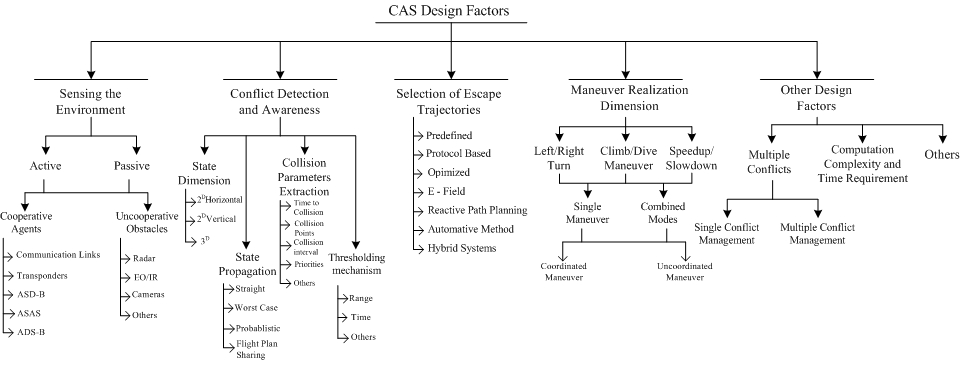
\includegraphics [width=1\textwidth] {09Rahim}
	\caption{Illustrates the main CAS design factors divisions with its subdivisions \cite{albaker2009survey}}
	\label{fig:09Rahim}
\end{figure*}

A framework for categorizing collision avoidance systems is presented in \cite{albaker2009survey}.  In this model, a collision avoidance system is conceptually broken down into different modules (Figure \ref{fig:09Rahim}).  A collision avoidance algorithm can be designed by including the conflict detection and escape trajectory selection, or conflict resolution, modules.  In this framework, a collision is defined as an instance in which two or more UAVs violate a minimum separation distance between each other, and a conflict occurs when two or more UAVs will enter a collision sometime in the future. In order to avoid collisions, it is necessary to first detect the corresponding conflict.  Therefore, conflict detection is a prerequisite of conflict resolution.

\subsection{Conflict detection and awareness}


\subsubsection{State Projection}

\begin{figure}[h]
	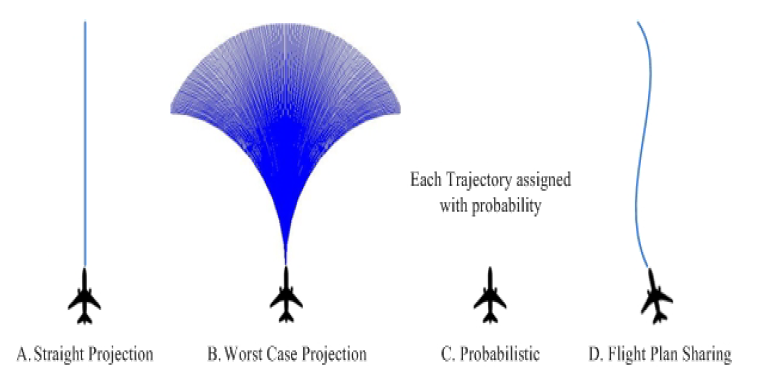
\includegraphics [width=1\columnwidth] {2009RahimProject}
	\caption{The four main types of state projection \cite{albaker2009survey}}
	\label{fig:09RahimProject}
\end{figure}

State projection refers to the method used to predict the future position of a UAV to detect conflicts. Figure \ref{fig:09RahimProject} provides a visual representation of each type of state projection and \cite{albaker2009survey} provides a description of each:

Nominal or straight projection traces the UAV's current trajectory and does not account for changing flight plans.  A conflict is detected if a UAV will collide with another UAV given that they both continue on their current headings.  However, straight projection is not reliable in cases where flight plans change frequently or for long projection times due to the fact that changed headings render previous predictions incorrect.

Worst-case projection traces all possible routes that a UAV could take and detects a conflict if any of these flight paths intersects with the flight path of another UAV.  Projection distance must be limited in this approach to prevent oversensitivity in conflict detection and to minimize computational time devoted to prediction.

Probabilistic projection is similar to worst-case projection in that it considers multiple variations on the current trajectory, but it adds the additional layer of considering the likelihood that the specific variation will occur.  

Flight plan sharing allows for a more direct detection of conflicts as it involves having multiple UAVs sharing portions of their planned trajectories with other nearby UAVs.  This method allows for accurate conflict detection, but presents the difficulty of actually transmitting these plans.  

\subsubsection{Collision Cone}

\begin{figure}[h]
	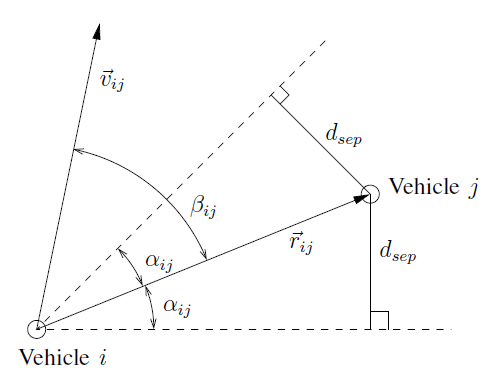
\includegraphics [width=1\columnwidth] {2008Kristi}
	\caption{The collision cone. A conflict is detected when velocity vector \begin{math}\vec{v_{ij}}\end{math} lies between the dotted lines \cite{lalish2008decentralized}}
	\label{fig:cone}
\end{figure}

The collision cone is a pairwise conflict detection system in which a system of two moving agents is converted into a system with a single agent and a static obstacle \cite{danielscollision}.  Collision cones can be used to determine if a pair of agents are in conflict, assuming that the agents will continue on their current trajectories.

A conflict is detected if the relative velocity vector lies within the collision cone. Mathematically, a minimum seperation distance, \begin{math}d_{sep} \end{math}, will be violated sometime in the future if \begin{math}\beta <  \alpha \end{math} where:
\newline
 \centerline{\begin{math} \beta = \ \angle\vec{v}  - \angle\vec{r}, \end{math}}
\newline
\centerline{\begin{math}\alpha = \arcsin(\frac{d_{sep}}{||\vec{r}||})\end{ math}}
\newline
\centerline{\begin{math} \vec{r} \end{ math} = relative position vector}
\newline
\centerline{\begin{math} \vec{v} \end{ math} = relative velocity vector}




\subsection{Conflict Resolution}


\subsubsection{Predefined}
In a predefined or rule based collision avoidance algorithm, certain rules define how a plane should maneuver given a specific situation.
One such implementation is detailed in \cite{sislak2006negotiation}. Potential collisions are categorized according to the angle of the collision as seen in Figure \ref{fig:06SislakID}; depending on the type of collision, each plane will execute a predefined escape maneuver. This decision is executed independently, with each plane detecting the collision from its point of view.  

This approach is relatively simple and easy to implement, taking up only as much processing power is needed to determine the type of collision. However, this approach is inherently static, and thus may not guarantee collision avoidance for special cases. In addition, because the maneuvers are arbitrarily predefined with no room for modifications, this approach may result in an inefficient escape maneuver when a more efficient one is available. 
\begin{figure}[h]
	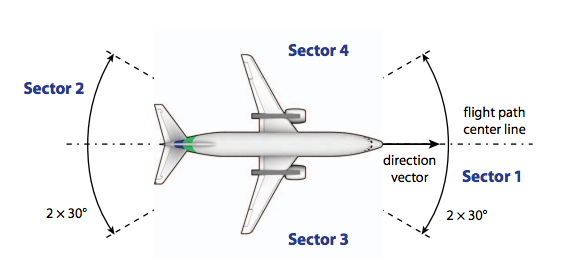
\includegraphics [width=1\columnwidth] {06SislakCollisionID}
	\caption{Categorizing collisions based on angle. \cite{sislak2006negotiation}}
	\label{fig:06SislakID}
\end{figure}
\subsubsection{Protocol based}

A negotiation based approach uses a predefined protocol to compromise and negotiate to achieve a mutually beneficial collision avoidance path. This approach assumes cooperative agents. The goal of such an approach is to find conflict-free flight paths for agents that are mutually beneficial.

One implementation of a protocol based collision avoidance algorithm is discussed in \cite{vsivslak2008agentfly}. The algorithm consists of four main steps - detection, negotiation set generation, path optimization, and execution. For the purposes of explaining the steps, a pair of conflicting agents is assumed.

Detection - Based on the flight plan data received from other agents, an agent can determine if a conflict is about to occur. Once a conflict is detected, the process of generating a negotiation set begins.

Negotiation Set Generation -
Each agent generates a set of possible maneuvers it could take. In the implementation described in \cite{vsivslak2008agentfly}, the author suggests six possible alternate trajectories - left/right turn, climb/descend, and speed up/slow down. Each possible trajectory is then marked with a utility value representing the desirability of the trajectory to the agent. The utility of a trajectory is determined by a utility function, defined as the difference between the cost of the trajectory and the cost of a fallback trajectory. Figure \ref{fig:05Wollkind} lists a number of possible cost functions \cite{wollkind2004automated}. The cost function encodes the preferences of each agent, and is taken into account during negotiations. The agent marks each possible trajectory with its calculated utility value and sends them over to the other agent.  

\begin{figure}[h]
	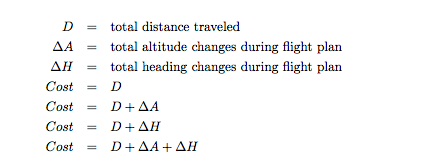
\includegraphics [width=1\columnwidth] {05WollkindCost}
	\caption{Cost functions for generating utility values. \cite{wollkind2004automated}}
	\label{fig:05Wollkind}
\end{figure}


Once an agent receives a set of possible paths from a conflicting agent, it will pair them up with its own set to make a new set of all possible pairs of paths both agents could take.  The resulting set is the preliminary negotiation set, and is made of up of deals, or pairs of possible paths. All deals in the preliminary negotiation set are then validated, with those generating further conflicts removed; the remaining pairs of non conflict generating paths make up the negotiation set. 

After generating the negotiation set, the next step is optimization. The “best” pair of paths must be found, taking into account the utility values associated with each deal. One possible way to find the best deal is to use the monotonic concession protocol (MCP), a incremental bargaining process described in  \cite{wollkind2004automated}  and \cite{zlotkin1989negotiation}. If no deal can be found, then a fallback deal must be executed. One option for the fallback deal is assuming the worst case scenario and finding a guaranteed safe trajectory no matter what the other agent does. 

The number of agents involved in the negotiation affects how and when these four steps are executed. For pairs of conflicting agents, each agent can either execute all four steps independently, or arbitrarily assign a master and slave to prevent repetition of work (Figure \ref{fig:07SislakMaster}). For conflicts involving more than two agents, the same pair-wise algorithm can be applied iteratively, or the master slave approach can be expanded to replace the master with a coordinator responsible for finding collision free paths for a party of planes.

\begin{figure}[h]
	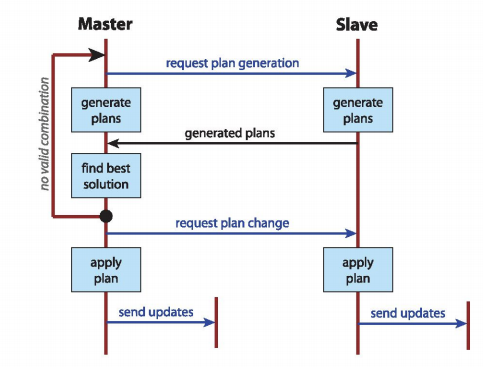
\includegraphics [width=1\columnwidth] {07SislakMasterSlave}
	\caption{Protocol based negotiations. \cite{vsivslak2008agentfly}}
	\label{fig:07SislakMaster}
\end{figure}


This approach's main benefit is that it negotiates a mutually beneficial path, and the measure of the benefit can be set by each agent. Each agent is able to inject its own preferences into the negotiating process. As a result, this approach can produce more efficient results and is more adaptable than a static, rule based method or a worst case method. However, the chattiness of the protocol requires more bandwidth for communications, and the algorithm itself requires more processing power depending on the number of agents involved. 

\subsubsection{Optimized}


The optimization approach to selecting escape trajectories involves formulating the problem in terms of constraints and cost functions.  Typically, the constraints are coupled with kinematic models of the planes and the cost functions are derived from a variety of metrics.  An escape trajectory can then be found by minimizing the cost function subject to the aforementioned constraints utilizing any optimization technique. Commonly used optimization techniques for this purpose include genetic algorithms, expert systems and fuzzy control.

Genetic algorithms search the solution space of possible paths using techniques inspired by evolution.  Genetic algorithms generally follow a set process, described as follows:  The first step in most genetic algorithms is to initialize a population, or a random set of initial solutions.  The algorithm then enters a loop in which it will iteratively mutate the most successful members of the population and continue to do so until a suitably fit solution is found \cite{siudynamic}.

Expert Systems make use of rule bases to decide how to categorize and resolve conflicts.  However, these systems require a large number of rules to recognize all type of conflicts and the resolutions to the types of conflict.  Once the rule base is established, its use of rules makes it relatively easy to understand. \cite{kuchar2000review}

Fuzzy control systems are modelled on fuzzy logic and follow a certain process.  In the first step, fuzzy values are created from numeric or “crisp” input.  The fuzzification of crisp input entails assigning descriptive tags to inputs that meet certain requirements.  For example, an altitude of 500-1000 meters could be classified as “high”.  A fuzzy control system can then apply a fuzzy rule base to this input to create a fuzzy output.  Finally, this output can be defuzzified to produce a flight plan. \cite{2012Fuzzy}

\subsubsection{E Field}


\begin{figure}
	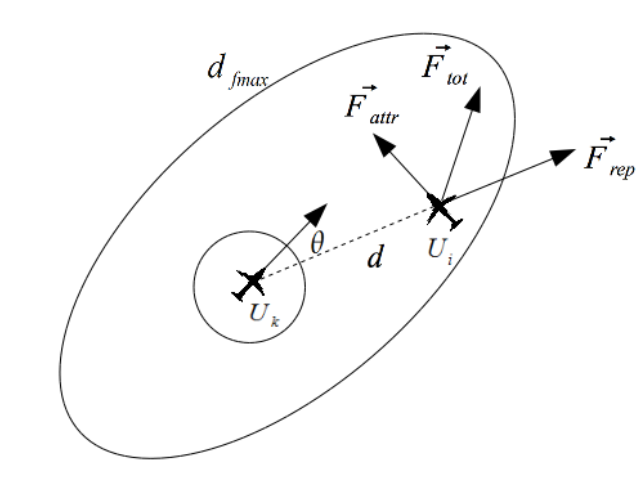
\includegraphics [width=1\columnwidth] {2011Ruchti}
	\caption{Calculating virtual forces acting on a UAV \cite{ruchti2011uav}}
	\label{fig:forceCalculation}
\end{figure}


The E-Field or APF (artificial potential field) approach to trajectory calculation involves modelling UAVs and their waypoints as charged particles.  UAVs are assigned the same charge so that they repel each other and waypoints are assigned an opposite charge so that their corresponding UAVs are attracted to them.  UAVs can then implicitly plan paths by summing attractive and repulsive forces to create the next desired heading.

Several factors need to be considered when designing an APF system.  One consideration is field shape.  While in reality, charged particles can affect other charged particles over any distance, there is little reason to implement such a field for UAVs in the context of collision avoidance.  If the APFs were to extend to a great distance, the contribution of force to the affected UAV would be negligible and would only use more computation time.  Therefore, it is often the case that limit functions are created to define a finite field shape around a UAV.  Another design consideration that should be taken into account is the field function.  Once a UAV enters another UAV's APF, the field function determines the magnitude (and possibly direction) of the repulsive force \cite{khatib1985real}.

There are several issues that arise when APFs are used for collision avoidance on unicycle UAVs.  If only APFs are utilized, then there is no method for resolving a head on collision between two UAVs with waypoints located behind each other.  This results from the fact that there exists no force in this configuration that would cause the UAVs to turn away from each other.  Another issue is looping.  Looping occurs when a UAV circles its goal waypoint and is unable to reach it due to turning constraints.  In a pure APF approach, the attractive force of a waypoint can provide the “centripetal force” needed to initiate looping.  It is possible to resolve both of these issues by explicitly identifying the situation and then applying the appropriate maneuver(s) to resolve the issue \cite{ruchti2011uav}.

APFs are a popular research topic and have been utilized in many different ways to implement collision avoidance.   \cite{ruchti2011uav}, \cite{balch2000social} and \cite{barnes2006swarm} all make use of APFs to govern swarming behavior.  Swarming, in this context, refers to the grouping of UAVs in a geometric fashion in response to a specific situation. Specifically,  \cite{ruchti2011uav} made use of flocking behaviours to limit competition between UAVs that had similar destinations.  \cite{chang2003collision} presents gyroscopic forces as another extension to APFs for collision avoidance.  In \cite{chang2003collision}, repulsive forces are replaced with a gyroscopic force that activates whenever two agents come within a certain distance of each other.

\begin{figure}
	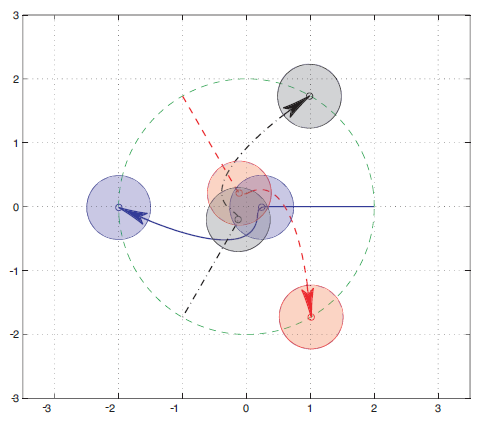
\includegraphics [width=1\columnwidth] {2003Chang}
	\caption{Gyroscopic forces allow three agents to spin free of their initial configuration and reach their antipodal destinations \cite{chang2003collision}}
	\label{fig:2003Chang}
\end{figure}

\section{Implementation}
\label{sec:implementation}

\subsection{APF Algorithm}

A modified APF algorithm was chosen to implement decentralized collision avoidance.  In this setup, each UAV is subject to attractive and repulsive forces which lead the UAV to its desired waypoint while avoiding collisions. The attractive force was modeled to have a constant magnitude with a direction facing the plane's goal waypoint. Repulsive forces, on the other hand, were calculated using a statically assigned field shape and field function on each plane. 

Statically assigned field shapes and functions enable each plane to calculate virtual forces using only the location and bearing of other planes.  The field shape was defined as an ovoid (INSERT\_FIGURE) and the field function was defined using bivariate normal functions (INSERT\_FIGURE), where the x and y coordinates would be relative to the plane generating the field.  A modular approach to APF assignment was taken, allowing users to define and make use of different field shapes and/or field functions. The correctness of the algorithm was then verified through simulation before it was ported to the hardware framework.


\subsection{Hardware}

The hardware used in this study consisted of the Bixler hobby plane and several control and communication devices used to automate its flight.  At the center of the control system is the ArduPilot, which enables stable flight between designated waypoints.  These waypoints are generated by our algorithm on a Raspberry Pi, which is a low cost microcomputer. Finally, we include XBee modules to enable wireless communication between UAVs and ground stations.  We connect the Raspberry Pi, ArduPilot and XBee  together using USB cables and communicate between the systems using the mavlink protocol.  Mavlink allows for sending and receiving c-structs over serial communication lines. See (INSERT\_DAVID\_PAPER) for a more detailed overview of the mavlink protocol and the custom messages used in our system.

\subsection{Architecture}

The decentralized collision avoidance framework developed in this work was implemented using ROS, or Robot Operating System. In ROS, processes are organized as “nodes”, and ROS provides methods for communication between nodes.   Our decentralized collision avoidance framework makes use of three nodes: the ardu, xbee and mover nodes.  The ardu and xbee nodes are responsible for handling communications between the ArduPilot and XBee devices respectively, while the mover node is responsible for forwarding waypoints to the ArduPilot and running the collision avoidance algorithm.  

These nodes communicate with each other by making use of “topics” which ROS provides access to. Topics have subscribers and publishers; subscribers read data from the topic and publishers post data to the topic. Figure \ref{fig:ROSDistributedSystem} provides a graphical representation of how the nodes communicate with each other using topics.  The four topics used for communicating between nodes are the my\_mav\_telem, gcs\_commands, all\_telemetry and ca\_commands topics.  

\begin{figure}  [h]
  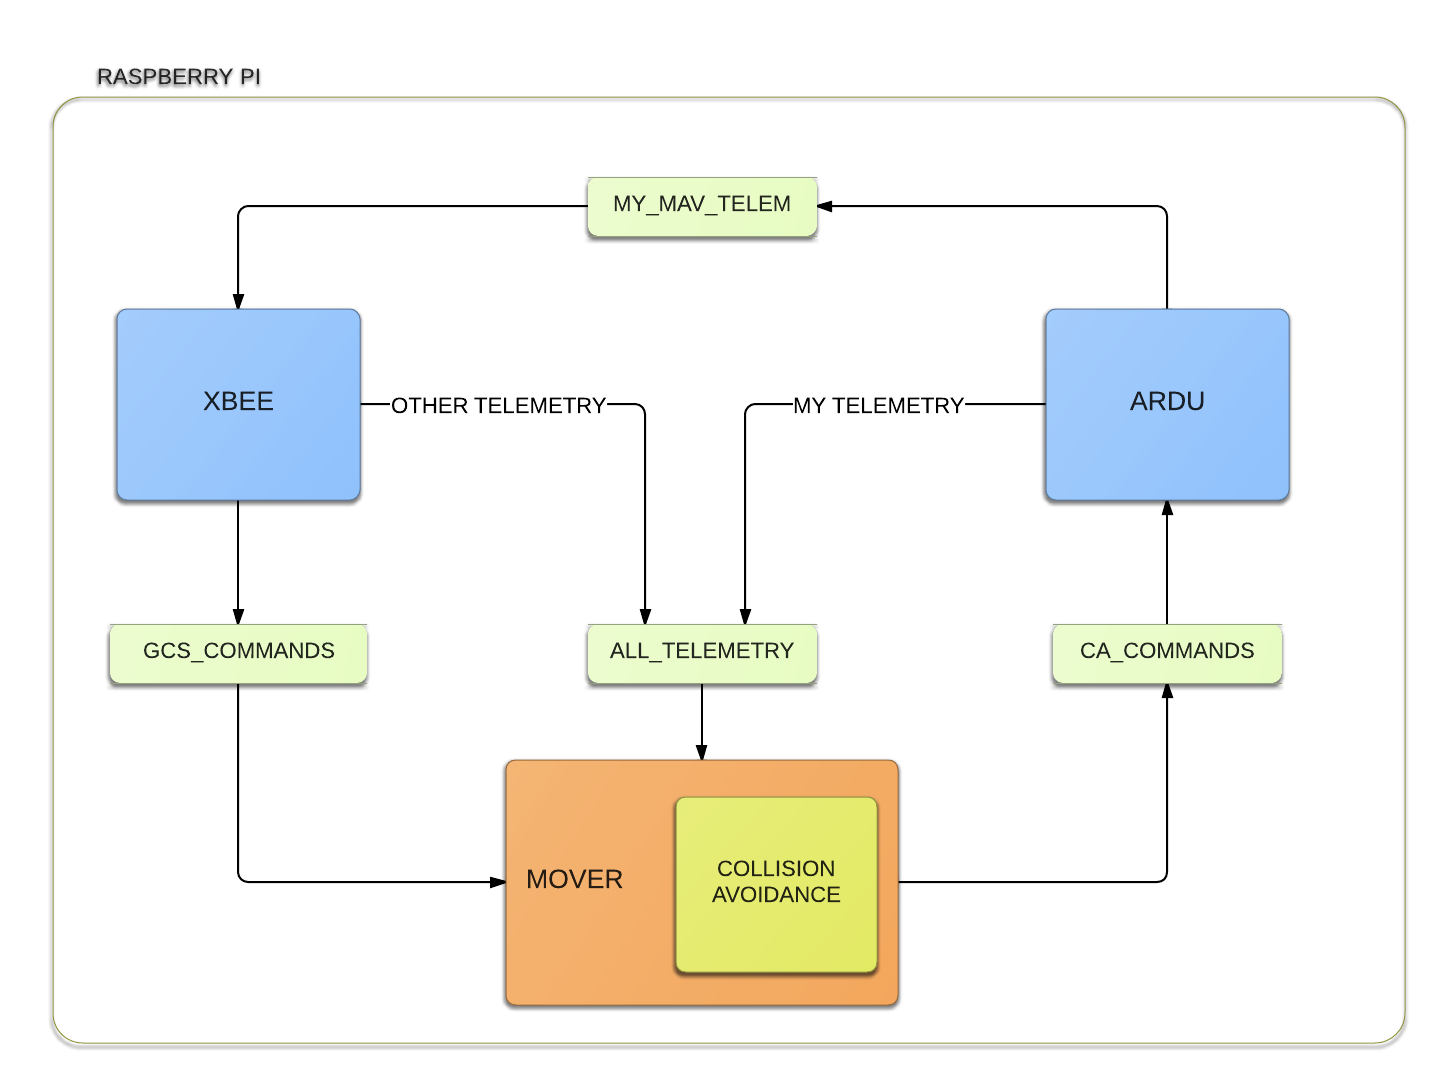
\includegraphics [width=1\columnwidth] {ROSDistributedSystem}
  \caption{Our framework architecture}
  \label{fig:ROSDistributedSystem}
\end{figure}
\subsubsection{Ardu}

The ardu node is responsible for handling communication between the Raspberry Pi and the ArduPilot system.  This entails receiving GPS information from the ArduPilot and forwarding waypoint commands to the ArduPilot. The ardu node accomplishes this by simultaneously listening to the ArduPilot's serial line and waiting for a message to be posted to ca\_commands. When the ardu node receives a telemetry update from the ArduPilot, it will publish this information to both the all\_telemetry topic (which is used by the mover node) and the my\_mav\_telemetry topic (which is used to send this telemetry to other UAVs).  

While the ardu node is listening for a telemetry update from the ArduPilot, it will also be waiting for a command to be published on the ca\_commands topic.  If a command is published on this topic, the ardu node will take the posted information, pack it into a mavlink message and then send it to the ArduPilot system using serial communication.  The ArduPilot will then set the new destination of the UAV to reflect the command.


\subsubsection{Xbee}

The xbee node is responsible for handling communication between the Raspberry Pi and the XBee module.  The XBee module communicates with other XBee modules by either receiving messages from a ground station and other UAVs or by sending out telemetry information to other systems.  Much like the ardu node, the xbee node simultaneously listens to the XBee module for a message and write to the XBee once a message is posted to the my\_mav\_telemetry topic.  

The xbee node can currently read and decode two types of mavlink messages: a telemetry update and a command.  If a telemetry update is read from the XBee module, the message is decoded and posted to the all\_telemetry topic (which is used by the mover node). If a command is read from the XBee module, it is decoded and posted to the gcs\_commands topic (which is also used by the mover node).  

In addition to reading from the XBee module, the xbee node also waits for a message to be posted to the my\_mav\_telem topic.  Once a message is posted to this topic, the xbee node will take the information, pack it to a mavlink message and perform a serial write to the XBee so that the telemetry information is sent out by the XBee module.


\subsubsection{Mover}
The mover node is responsible for generating waypoints to send to the ArduPilot. 
This node operates by taking in telemetry messages and ground station control commands, then periodically forwarding waypoints to ca\_commands so that they can be sent to the ArduPilot.  Input to this node is taken from either the gcs\_commands topic or the all\_telemetry topic.  Messages from the gcs\_commands topic specify a goal waypoint that the UAV should eventually aim to reach while running collision avoidance.  Messages from the all\_telemetry topic, on the other hand, contain GPS updates from all other UAVs (including the plane running this framework). Depending on the state that the mover node is in (see section \ref{sec:statebased}), the forwarded waypoint will be either a collision avoidance waypoint or the goal waypoint. 
The waypoint is forwarded to the ardu node through the ca\_commands topic at a preset rate so that the ArduPilot is not flooded with commands.

\subsubsection{Collision Avoidance}
One of the requirements of our system is that it must be modular, such that users can implement their own distributed collision avoidance algorithms within our framework. 
This was accomplished by encapsulating the collision avoidance logic in the Collision Avoidance class (CA) inside the mover node. Every time a telemetry update is received by mover, the avoid function in CA containing the user specified collision avoidance algorithm is executed. Using the incoming telemetry information, the avoid function generates a collision avoidance waypoint which is then forwarded to the ArduPilot by the mover node.

Encapsulating the collision avoidance logic in its own class provides two main benefits -  users can implement their collision avoidance algorithm and any other needed variables in a self contained manner, and different collision avoidance algorithms can be swapped easily. 

\subsection{Ease of Testing}

For ease of testing, we introduce two features implemented in our framework: state based command forwarding and a pseudo ground control station.
\subsubsection{State Based Command Forwarding}
\label{sec:statebased}

\begin{figure}  [h]
  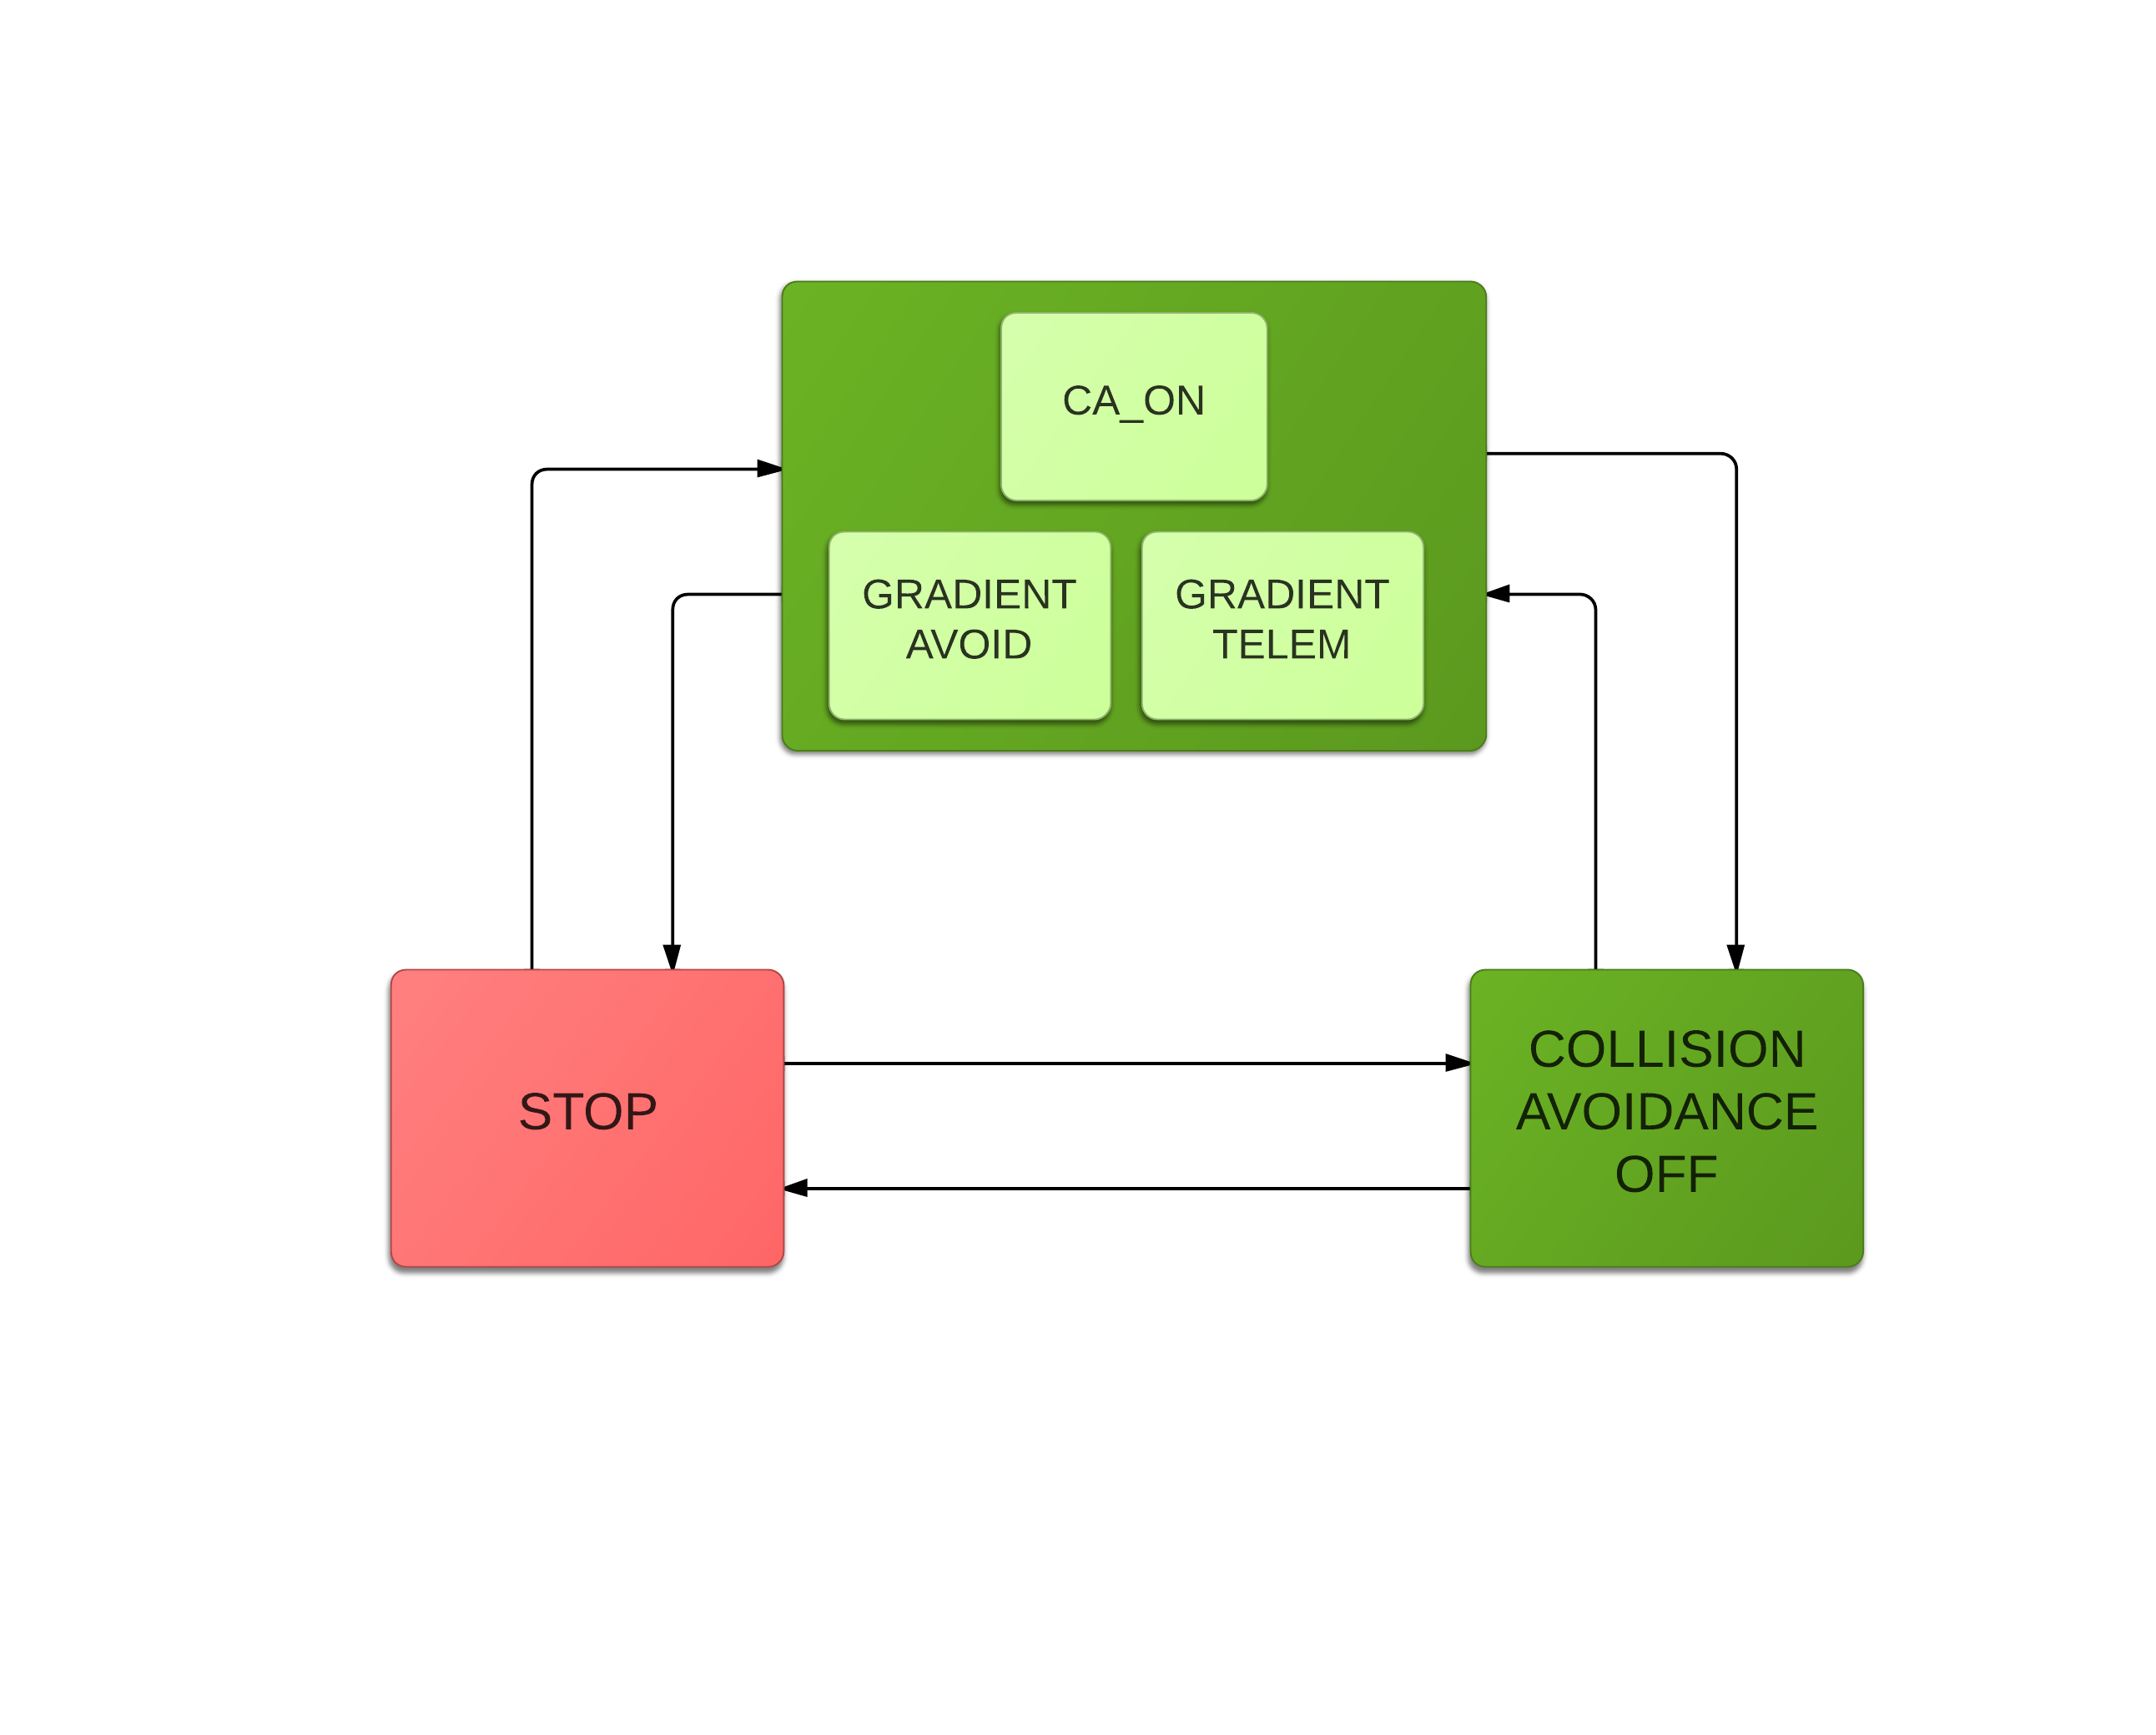
\includegraphics [width=1\columnwidth] {stateDiagramv2}
  \caption{State based command forwarding}
  \label{fig:statebased}
\end{figure}

The mover node operates in three main states that dictate what type of command waypoint is sent to the ArduPilot, illustrated in Figure \ref{fig:statebased}. 
In the stop state (ST\_RED), no commands are published by mover and sent to the ArduPilot. This state is in place to ensure manual remote control mode of the ArduPilot will not be overridden by any unnecessary commands from mover.
In the collision avoidance off (CA\_OFF) state, the mover node simply forwards goal waypoints to the ArduPilot, without using any collision avoidance. In this mode, the behavior of the plane is the same as if there were only an ArduPilot receiving commands from the ground control station, and no Raspberry Pi in the middle. In the collision avoidance on state (CA\_ON), the mover node forwards collision avoidance waypoints generated by the CA algorithm. 

Within the CA\_ON state, there are two further substates used to simplify testing. The tests substitute the goal waypoint instead of a generated collision avoidance waypoint at different levels, or gradients, of the telemetry callback. The first is the gradient telemetry state (GRADIENT\_TELEM); when a telemetry message is received, the goal waypoint is added to the collision avoidance queue instead of a collision avoidance waypoint. The second state is the gradient avoid state(GRADIENT\_AVOID); it is similar to the original CA\_ON state in that it calls CA's avoid function, but the goal waypoint is substituted from within CA's avoid function. The purpose behind these substates is to allow for further testing of the core framework separate from the collision avoidance algorithm.

State changes are triggered when ground station commands with specially defined latitude and longitude are sent. This feature works in conjunction with the gcs\_routing node, explained in the next section.


\subsubsection{Pseudo Ground Control Station}

The gcs\_routing node offers a method for integrating a pseudo ground control station for testing our framework.  This node operates much like the xbee node, but adds in the ability to send user-specified commands and telemetry to UAVs running our framework.  The user can choose to publish a specific message to either the my\_mav\_telem topic or the gcs\_commands topic to send out a telemetry message or a waypoint command.  The gcs\_routing node responds to messages posted on these two topics by packing the messages into the correct mavlink format and sending the message through XBee to other UAVs.  When switching execution states, the user publishes a message to the gcs\_commands topic with specific latitudes and longitudes that correspond to the desired state.  

The gcs\_routing node can also be run with the ardu node and/or the mover node to further expand testing capabilities.  If the ardu node were to be run, the ArduPilot would have to be tethered to the ground control station, leaving the connected ArduPilot with a lower altitude.  However, this ArduPilot could then simulate another plane by automatically generating telemetry updates, and can then be positioned so that the plane in the air should avoid it.  Additionally, the mover node could be run on the ground station to ensure that the grounded ArduPilot would also avoid the collision as if it were in the air.



\section{Results}
\label{sec:results}

We tested our framework by running communications tests on the ground and by flying the Bixler with the aforementioned hardware. In the communications test, we were able to successfully receive and send all messages that would come into and out of the Raspberry Pi.  The xbee node can successfully receive and decode messages that were sent by other XBees and can forward messages to the appropriate topics within the framework.  In addition, the ardu node can successfully read telemetry information from the ArduPilot and can send commands to the ArduPilot such that the ArduPilot updates its destination to be this command.  Finally, the mover node correctly follows the state based behaviour that was previously outlined.  

The flight tests we conducted made use of one airborne UAV and one UAV tethered to a ground station so that state-based testing could be used.  The tethered UAV served the purpose of generating telemetry updates automatically. In addition, the tethered UAV allowed us to visualize the location of the airborne UAV relative to the location of the tethered UAV. In conducting the flight tests, we cycled through each of the flight states to ensure each of them were working correctly.

 In the CA\_OFF state (mode that forwards goal waypoint) the Bixler was able to successfully fly to its goal waypoint.  This verified that the framework does communicate correctly with the ground control station and that the communication is done in such a way that it does not disrupt the functionality of the ArduPilot. In addition, we were able to successfully switch between flight states in mid flight, which allowed for the activation of our algorithm by moving to the CA\_ON state. 

Our APF algorithm was tested in the air by means of a two step process.  The first step taken was that our APF algorithm would be activated when there were no other simulated or real UAVs in the airspace.  This test verified that our algorithm would correctly direct the UAV to its goal waypoint by making use of attractive forces.  When run on the airborne UAV, the algorithm correctly directed the UAV to the appropriate goal waypoint.  The second test performed involved sending out telemetry information for both real and simulated planes so that the UAV in the air would experience repulsive forces.  When run on the airborne UAV, the algorithm successfully generated avoidance waypoints that directed the airborne UAV away from both the tethered UAV and the simulated UAVs. 

In the ST\_RED state, we were able to successfully regain manual control of the plane and land it safely. Finally, the flight behaviour of the Bixler was only slightly changed by the weight of the additional hardware, and the Bixler was still able to move to the correct destination without needing to adjust control parameters.

\section{Conclusion}
\label{sec:conclusion}
%The conclusion goes here.

Decentralized collision avoidance algorithms are especially suited to UAVs' inherent mobility and range, as they reduce the dependency on a ground control station that centralized algorithms require. However, decentralized collision avoidance algorithms require an efficient surrounding framework. A lightweight, modular framework for testing different distributed collision avoidance algorithms was presented in this paper. Our framework was implemented using an existing, modified APF algorithm on a commercially available drone outfitted with an XBee, Raspberry Pi, and ArduPilot. The functionality of our framework, both with and without collision avoidance, was verified through integration testing as well as flight testing.

\section{Future Work}
\label{sec:future work}
\subsection{Simulating GPS data}
Throughout our testing period, the imprecision and drift of real GPS data made it very difficult to accurately test our algorithm within our framework. In addition, the long setup time and travel required for performing test flights made frequent flight tests impractical. This problem can be addressed in two possible ways - either through some sort of visualization of real time GPS data, similar to how the existing simulator works, or faking more reliable GPS data. Future work could include using the ArduPilot mission planner's simulated GPS capabilities to more efficiently test distributed collision avoidance algorithms without having to physically fly the planes or bring them outside. 

\subsection{Integration with Ground Control}
During flight tests, our framework was mainly tested with our custom gcs\_routing station. Full integration of our framework with the existing ground control station and simulator would allow for easier testing, as the simulator could visually display plane location. In addition, distributed collision avoidance algorithms could be tested with a combination of simulated planes and real planes to minimize loss of hardware. As mentioned in the above section, combining the ArduPilot mission planner's simulated GPS with integration into the existing ground control station would also allow use of the existing testing infrastructure.

\subsection{XBee Networking}

One limitation that our work was subject to was that the XBees we used to network our devices were set up so that only pairwise connections were reliable enough to be used.  This resulted in only using two XBees in any particular setup.  Efforts at adding a third XBee and implementing communication through broadcasts resulted in packet loss and packet clustering.  If this system is to be implemented on more than two devices, work needs to be done to configure the XBees so that a reliable n to n network can be established. 


% An example of a floating figure using the graphicx package.
% Note that \label must occur AFTER (or within) \caption.
% For figures, \caption should occur after the \includegraphics.
% Note that IEEEtran v1.7 and later has special internal code that
% is designed to preserve the operation of \label within \caption
% even when the captionsoff option is in effect. However, because
% of issues like this, it may be the safest practice to put all your
% \label just after \caption rather than within \caption{}.
%
% Reminder: the "draftcls" or "draftclsnofoot", not "draft", class
% option should be used if it is desired that the figures are to be
% displayed while in draft mode.
%
%\begin{figure}[!t]
%\centering
%\includegraphics[width=2.5in]{myfigure}
% where an .eps filename suffix will be assumed under latex, 
% and a .pdf suffix will be assumed for pdflatex; or what has been declared
% via \DeclareGraphicsExtensions.
%\caption{Simulation Results}
%\label{fig_sim}
%\end{figure}

% Note that IEEE typically puts floats only at the top, even when this
% results in a large percentage of a column being occupied by floats.


% An example of a double column floating figure using two subfigures.
% (The subfig.sty package must be loaded for this to work.)
% The subfigure \label commands are set within each subfloat command, the
% \label for the overall figure must come after \caption.
% \hfil must be used as a separator to get equal spacing.
% The subfigure.sty package works much the same way, except \subfigure is
% used instead of \subfloat.
%
%\begin{figure*}[!t]
%\centerline{\subfloat[Case I]\includegraphics[width=2.5in]{subfigcase1}%
%\label{fig_first_case}}
%\hfil
%\subfloat[Case II]{\includegraphics[width=2.5in]{subfigcase2}%
%\label{fig_second_case}}}
%\caption{Simulation results}
%\label{fig_sim}
%\end{figure*}
%
% Note that often IEEE papers with subfigures do not employ subfigure
% captions (using the optional argument to \subfloat), but instead will
% reference/describe all of them (a), (b), etc., within the main caption.


% An example of a floating table. Note that, for IEEE style tables, the 
% \caption command should come BEFORE the table. Table text will default to
% \footnotesize as IEEE normally uses this smaller font for tables.
% The \label must come after \caption as always.
%
%\begin{table}[!t]
%% increase table row spacing, adjust to taste
%\renewcommand{\arraystretch}{1.3}
% if using array.sty, it might be a good idea to tweak the value of
% \extrarowheight as needed to properly center the text within the cells
%\caption{An Example of a Table}
%\label{table_example}
%\centering
%% Some packages, such as MDW tools, offer better commands for making tables
%% than the plain LaTeX2e tabular which is used here.
%\begin{tabular}{|c||c|}
%\hline
%One & Two\\
%\hline
%Three & Four\\
%\hline
%\end{tabular}
%\end{table}


% Note that IEEE does not put floats in the very first column - or typically
% anywhere on the first page for that matter. Also, in-text middle ("here")
% positioning is not used. Most IEEE journals/conferences use top floats
% exclusively. Note that, LaTeX2e, unlike IEEE journals/conferences, places
% footnotes above bottom floats. This can be corrected via the \fnbelowfloat
% command of the stfloats package.







% conference papers do not normally have an appendix


% use section* for acknowledgement
\section*{Acknowledgment}
ACKNOLWEDGEMENTS



% trigger a \newpage just before the given reference
% number - used to balance the columns on the last page
% adjust value as needed - may need to be readjusted if
% the document is modified later
%\IEEEtriggeratref{8}
% The "triggered" command can be changed if desired:
%\IEEEtriggercmd{\enlargethispage{-5in}}

% references section

% can use a bibliography generated by BibTeX as a .bbl file
% BibTeX documentation can be easily obtained at:
% http://www.ctan.org/tex-archive/biblio/bibtex/contrib/doc/
% The IEEEtran BibTeX style support page is at:
% http://www.michaelshell.org/tex/ieeetran/bibtex/
\bibliographystyle{IEEEtran}
% argument is your BibTeX string definitions and bibliography database(s)
\bibliography{mybib}
%
% <OR> manually copy in the resultant .bbl file
% set second argument of \begin to the number of references
% (used to reserve space for the reference number labels box)


% that's all folks
\end{document}


